\documentclass{scrbook}

\usepackage[dvipsnames,table]{xcolor}
\usepackage{amsmath, amssymb, amsfonts, amsthm}
\usepackage{cancel}
\usepackage[ngerman]{babel}
\usepackage{enumerate}
\usepackage{hyperref}
\usepackage[utf8]{inputenc}
\usepackage[a4paper,left=2cm,right=2cm,top=1.5cm,bottom=1cm,includeheadfoot]{geometry}
\usepackage{graphicx}
\usepackage[amssymb]{SIunits}
\usepackage{tikz}

\setlength{\parindent}{1cm}

\newtheorem{goal}{Ziel}

\title{Skript - Einführung in die Astronomie und Astrophysik}
\author{Transkribiert von\\ Martine Lenders und Robin Nehls}

\begin{document}
\maketitle

\tableofcontents

\part{Klassische Astronomie}
\chapter{Koordinatensysteme, Zeit, Sternörter}
\section{Grundlagen der sphärischen Astronomie}
\subsection{Bezugssysteme}
\begin{itemize}
    \item Orientierung: Konstellationen am Himmel\\
        $\rightarrow$ \textbf{Problem:} systematische Bewegung\\
        $\Rightarrow$ \textbf{Bezugssystem mit Fixpunkten}
    \item Symmetrie $\mapsto$ Kuppelkoordinaten \\
        $\hookrightarrow$ Fixierung an Drehimpulsvektoren
    \item Koordinatenursprung im Schwerpunkt
\end{itemize}

\subsection{Äquatorialsystem}
\begin{goal}
    Positionsbeschreibung im Inertialsystem, Fixierung an Drehimpulsvektoren
    der Erdbewegung
\end{goal}

\begin{description}
    \item[Eigendrehimpuls]  $\vec n_e$
    \item[Bahndrehimpuls]   $\vec n_b$
    \item[Einheitsvektor in Richtung Frühlingspunkt]   $\vec n_{\vernal}$
\end{description}

\begin{equation}
    (\vec n_e \times \vec n_b) = \vec n_{\vernal}
\end{equation}

\begin{definition}
    Orthonormalsystem Äquatorialsystem: $(\vec n_e$, $\vec n_{\vernal}$, $(\vec n_e \times \vec n_{\vernal}))$
\end{definition}

\begin{center}
    \begin{tikzpicture}[scale=4,tdplot_main_coords]
        \pgfmathsetmacro{\rvec}{0.8}
        \pgfmathsetmacro{\alphavec}{60}
        \pgfmathsetmacro{\deltavec}{30}

        \coordinate (O) at (0,0,0);
        \tdplotsetcoord{S}{\rvec}{\deltavec}{\alphavec}

        \draw [->, thick] (O) -- (1, 0, 0) node[anchor=north east] {$\vec n_{\vernal}$};
        \draw [->, thick] (O) -- (0, 1, 0) node[anchor=north west] {$(\vec n_e \times \vec n_{\vernal})$};
        \draw [->, thick] (O) -- (0, 0, 1) node[anchor=south] {$\vec n_e$};

        \tdplotsetrotatedcoords{60}{40}{30}

        \tdplotdrawarc[dashed]{(O)}{1.5}{0}{360}{anchor=south west}{Himmelsäquator}
        \draw [->] (O) -- (S) node [pos=0.5, anchor=south east] {$r$};
        \draw [dotted] (O) -- (Sxy);
        \draw [dotted] (Sxy) -- (S) node [anchor=south west] {$\vec n$};
        \tdplotdrawarc[dotted]{(O)}{0.3}{0}{\alphavec}{anchor=south}{$\alpha$}
        \tdplotsetthetaplanecoords{\alphavec}
        \tdplotdrawarc[dotted, tdplot_rotated_coords]{(O)}{0.2}{\deltavec}{90}{anchor=east}{$\delta$}
    \end{tikzpicture}
    \[ \vec n = \sin \delta \cdot \vec n_e + \cos \delta \cdot \cos \alpha \cdot \vec n_{\vernal} + \cos \delta \cdot \sin \alpha \cdot (\vec n_e \times \vec n_{\vernal}) \]
\end{center}

\begin{itemize}
    \item $\alpha$: Rektaszension [$^\mathrm{h}$, $^\mathrm{m}$, $^\second$]
    \item $\delta$: Deklination [$\degree$, $\arcminute$, $\arcsecond$]
    \item Umrechnung: $360\degree \mathrel{\hat=} 24^\mathrm{h} \Leftrightarrow 15\degree \mathrel{\hat=} 1^\mathrm{h}$
    \item \textbf{Position eines astronomischen Objektes}: $\boxed{(\alpha, \delta)\text{-Angabe}}$
    \item Koordinaten Frühlingspunkt: $(0, 0)$
\end{itemize}

\chapter{Himmelsmechanik}
\section{Kinematik}
\subsection*{vor Newton}
\begin{description}
    \item[Aufgabe] genaue Beschreibung der scheinbaren Bewengung
        \begin{itemize}
            \item \emph{nicht} die Erklärung/das Verständnis des zugrunde
                  liegenden Sachverhaltes (Gesetztes)
        \end{itemize}
    \item[speziell] scheinbare Planetenbahnen $\rightarrow$ Mars
        \begin{center}
            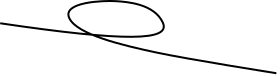
\includegraphics[width=.3\textwidth]{img/ptolemaeus_mars.pdf}
        \end{center}
    \item[Modelle]
        \begin{itemize}
            \item \textsc{Ptolemäus:}
                \begin{itemize}
                    \item Geozentrisch (Erde im Zentrum)
                    \item Planeten auf Epizykelbahnen
                \end{itemize}
            \item \textsc{Kopernikus:}
                \begin{itemize}
                    \item Heliozentrisch (Sonne im Zentrum)
                    \item \emph{Kreisbahnen}
                \end{itemize}
        \end{itemize}
    \item[Enscheidung] z. B. Planetenphasen der inneren Planeten\\
        $\Rightarrow$ Kopernisches Weltbild
\end{description}
\begin{itemize}
    \item \textsc{Kepler:} Messung d. Marsbahnen (T. \textsc{Brahe})\\
          $\Rightarrow$ \textsc{Kepler}'sche Gesetze (empirisch)
          \begin{enumerate}
              \item Ellipsen, Sonne in einem Brennpunkt
              \item Flächensatz $\Leftrightarrow$ Drehimpulserhaltung \\
                    Radiusvektoren überstreichen in gleicher Zeit gleiche Flächen,\\
                    d. h. Flächengeschwindigkeit = $\mathbf{const}$
              \item Umlaufzeiten/Abstände ($a$: Halbachse, $T$: Umlaufzeit)
                      \[ \frac{a^3}{T^2} \sim \mathbf{const} \]
          \end{enumerate}
\end{itemize}

\section{Newton'sche Mechanik}
\textsc{Newton}'sche Axiome:
\begin{enumerate}[(i)]
    \item Trägheitsgesetz (Masse konstant, vergl. spezielle Relativitätstheorie):
        \[ \vec p = m \vec v = m \dot{\vec{r}} = m \frac{d}{dt} \vec r \]
    \item Impulsänderung durch Krafteinwirkung:
        \[ \frac{d}{dt} \vec p = \dot{\vec p} = \vec F = m \ddot{\vec r} = m \frac{d^2}{dt^2} \vec r = m \vec a \]
    \item Actio = Reactio:
        \[ \vec F_{ik} = -\vec F_{ki} \]
\end{enumerate}

\end{document}
